\tikzstyle{block} = [draw, fill=white!20, rectangle]
\tikzstyle{sum} = [draw, fill=white!20, circle, node distance=1cm]
\tikzstyle{input} = [coordinate]
\tikzstyle{output} = [coordinate]

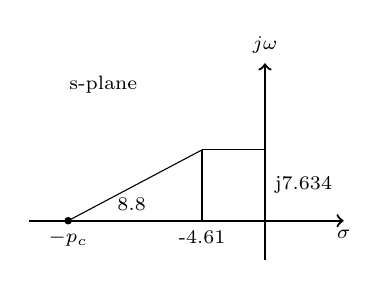
\begin{tikzpicture}
    \draw[thick,->] (-3,0) -- (1,0);
    \draw[thick,->] (0,-0.5) -- (0,2);
    \draw (-0.8,0) -- (-0.8,0.9);
    \draw (0,0.9) -- (-0.8,0.9);
    \draw (-2.5,0) -- (-0.8,0.9);
    \draw[fill] (-2.5,0) circle [radius=0.04];
    
    \node[below] at (-2.5,0) {\scriptsize $-p_c$};
    \node[right] at (0,0.45) {\scriptsize j7.634};
    \node[below] at (-0.8,0) {\scriptsize -4.61};
    \node[below] at (1, 0) {\scriptsize $\sigma$};
    \node[above] at (0, 2) {\scriptsize $j\omega$};
    \node[above right] at (-2, 0) {\scriptsize $8.8\degree$};
    \node[above left] at (-1.5, 1.5) {\scriptsize s-plane};
    
\end{tikzpicture}   